%\subsection{Introduction}
\label{sec:Introduction}
Characterizing the role of culture in shaping cognition is one of the fundamental questions in cognitive science \parencite{barrett2020towards, henrichWeirdest2010}. Culture is influenced by many factors, including language \parencite{blasi2022over,kramsch2014language}, values \parencite{inglehart2000world,triandis2018individualism}, and economy \parencite{fine2016world,henrich2001search}. More recently, globalization, as well as the spread of information over the internet, have had an increasing impact on societies around the world \parencite{barrett2020towards, pieterse2019globalization}. Here, we study the effect of globalization on cognition using the paradigmatic case of color terms.

Color concepts are a classic domain for studying the interaction between language and perception across cultures \parencite{whorfLanguage2012}. This is exemplified by the seminal works of \textcite{berlinBasic1969} and the World Color Survey (WCS; \textcite{kayWorld2016} 2016) on characterizing basic color concepts in written and unwritten languages, respectively. Their key findings are that a) speakers of different languages produce different color maps when describing the same set of colors using their respective basic color terms and b) there is a large overlap between color maps in languages that share the same number of basic color terms.  These findings have been elaborated on in numerous studies (e.g., German: \textcite{zollingerWhy1984}; Greek: \textcite{thierryUnconscious2009}; Turkish: \textcite{ozgenTurkish1998}) and they were linked to a variety of principles such as statistical learning and information-theoretic constraints \parencite{regierLanguage2009, zaslavskyEfficient2018}.

Surprisingly, there are no large-scale, standardized, contemporary color-naming data at a global scale. The largest color-naming study, the World Color Survey \parencite{kayWorld2016}, had fairly standardized procedures for each language, but focused on collecting data for unwritten languages, mostly from small-scale societies. 
%Many other contemporary studies that did collect some data of written languages are either not publicly available or cover only a few languages, each with different methodologies (for example \textcite{lindseyColor2014,al-rasheedFurther2014, daviesBasic1994, kurikiModern2017, ozgenTurkish1998, thierryUnconscious2009, zollingerWhy1984,winawerRussian2007,berlinBasic1969}). 
Many studies examined a small number of specific languages (e.g., German: \textcite{zollingerWhy1984}; Greek: \textcite{thierryUnconscious2009}; Turkish: \textcite{ozgenTurkish1998}), but they do not have a standardized procedure, have limited color coverage (e.g \parencite{winawerRussian2007}), and are likely to be out of date now \parencite{al-rasheedFurther2014, berlinBasic1969,kurikiModern2017, ozgenTurkish1998, thierryUnconscious2009, zollingerWhy1984}.
Furthermore, even if color-naming data were available for written languages, it is still difficult to define a suitable control class that could reflect high levels of globalization and multilingualism. Interestingly, it was assumed that globalization effects might resolve cross-cultural differences in color terminology, which is also a reason why there was low interest in studying languages with many speakers.
As a result, the effect of globalization on color naming has yet to be tested at scale. 

To address this, we leverage Lucid\footnote{\url{https:/www.cint.com}}, a nontraditional diverse recruiter, to collect color-naming data for 25 languages with a unified methodology.  The Lucid recruiter provides access to significantly larger participant pools from a diverse range of countries and languages than most traditional recruitment platforms such as Amazon Mechanical Turk or Prolific.  As an additional feature of this research we compared the collected human data with data elicited from multilingual state-of-the-art Large Language Models (LLMs, here GPT-4; \textcite{achiam2023gpt}) and Vision Language Models (VLMs, here GPT-4V) that have been trained on virtually all digitally available text in many languages (as well as a large number of images in the case of the VLMs). These models are assumed to be a control class that simulates the ultimately globalized agent (highly multilingual, heavily exposed to the internet, with access to digital content from around the world).
%% HERE IS AN STARTIGN ON THIS TEXT

This dissertation describe a project aiming to re-investigate color terms from a global perspective. Before describing the new set of experiment, I start by providing background vision and perception. Than I follow up with xxx and xxx....... [FEEL IN HERE]



% We also use multilingual state-of-the-art Large Language Models (LLMs, here GPT-4; \textcite{achiam2023gpt}) and Vision Language Models (VLMs, here GPT-4V) that have been trained on virtually all digitally available text in many languages (as well as a large number of images in the case of the VLMs) as a control class to simulate the ultimately globalized agent (highly multilingual, heavily exposed to the internet, with access to digital content from around the world).

% We find that even among internet users, we still see structural variation in the number of basic color terms and maps across languages. 
% Even when using LLMs and VLMs to simulate the limits of globalization, we see analogous differences when the agents are queried in different languages. 
% Taken together, our findings demonstrate how online experiments can be coupled with recent advances in machine learning to better understand classical questions in cognitive science. We provide an interactive visualization of our data here:
% \url{https://global-colors.s3-eu-central-1.amazonaws.com/index.html}.

% Naming different colors and therefore subdividing color space into discrete categories is an intuitive process.
% However, it is well known that the number of color terms and their related location in color space differs strongly across languages.
% Hence, although people around the globe see the same thing, they still use different systems of categories to name it.
% \begin{figure}
%     \centering
%     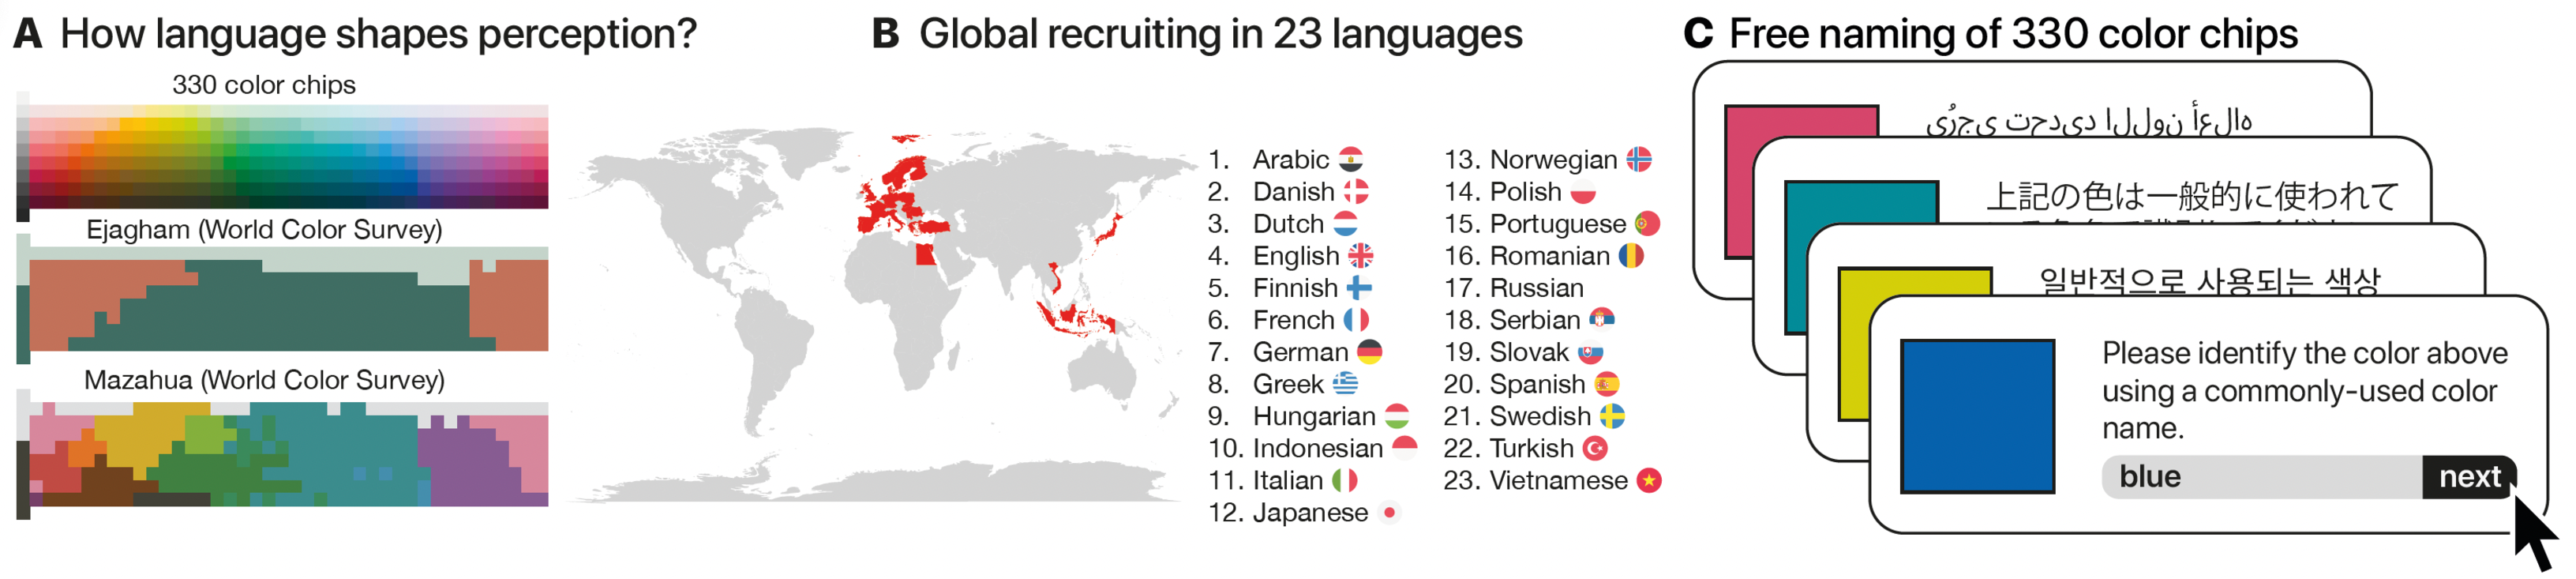
\includegraphics[width=1\linewidth]{images/approach.pdf}
%     \caption{Enter Caption}
%     \label{fig:enter-label}
% \end{figure}
% The fact that color terms have a direct physical correspondence makes them an excellent domain to study the relationship of language and thought.
% According to the Sapir-Whorf hypothesis, we perceive and interact with our environment through the filters and categories of our language.


% Are thoughts and perception shaped by language or the other way round?



% % relative linguistic


% % color domain
% - good as it directly refers to a physical representation of meanings

% % lack of industrialized languages

% % encoded in the language -> encoded in LLM`s